\documentclass[11pt]{article}
\usepackage[margin=1in]{geometry}
\usepackage{mathptmx}
\usepackage[T1]{fontenc}
\usepackage{microtype}
\usepackage{amsmath, amssymb}
\usepackage{tabularx}
\usepackage{graphicx}
\usepackage{booktabs}
\usepackage{xcolor}
\usepackage{listings}
\usepackage{enumitem}
\usepackage[hypcap=false]{caption}
\usepackage{subcaption}
\usepackage[hidelinks]{hyperref}

% --------------------------------------------------------------------------------------------
% Listings and Document Formatting
% --------------------------------------------------------------------------------------------
\definecolor{codebg}{rgb}{0.98, 0.98, 0.98}
\definecolor{codecomment}{rgb}{0.25, 0.50, 0.35}
\definecolor{codekeyword}{rgb}{0.0, 0.20, 0.70}
\definecolor{codenumbers}{rgb}{0.55, 0.55, 0.55}
\definecolor{codestring}{rgb}{0.70, 0.10, 0.10}

\lstdefinestyle{gostyle}{
    backgroundcolor=\color{codebg},
    commentstyle=\color{codecomment}\itshape,
    keywordstyle=\color{codekeyword}\bfseries,
    stringstyle=\color{codestring},
    numberstyle=\tiny\color{codenumbers},
    basicstyle=\ttfamily\scriptsize,
    breaklines=true,
    numbers=left,
    numbersep=5pt,
    frame=single,
    rulecolor=\color{black!20},
    tabsize=4,
    xleftmargin=1.2em,
    framexleftmargin=1.2em,
    morekeywords={package,import,func,type,struct,interface,var,const,return,if,else,for,range,go,select,case,default,switch,defer,chan,make,len,cap,copy,nil,true,false,int,int64,bool,string,float64}
}
\lstset{style=gostyle}

\setlist[itemize]{leftmargin=1.4em, itemsep=0.08em, topsep=0.08em}
\setlist[enumerate]{leftmargin=1.4em, itemsep=0.08em, topsep=0.08em}

% --------------------------------------------------------------------------------------------

\begin{document}

\begin{center}
    
\includegraphics[width=0.30\textwidth]{VNIT_logo.jpg}\\[1.5cm]
    
    {\large \textbf{Group Members}}\\[0.3cm]
    \begin{tabular}{l c l}
        Student 1: Gaurav Acharya & --- & [MT26MCS024] \\
        Student 2: Sandeep & --- & [MT26MCS032]
    \end{tabular}
    
    \vspace{1.0cm}
    
    {\large \textbf{Guide Name}}\\[0.3cm]
    Dr. A. S. Mokhade
    
    \vspace{1.0cm}
    
    {\large \textbf{Practical Title:}}\\[0.3cm]
    CSP502 Software Lab-I:\\[0.15cm]
    Practical 6: Concurrency Meets Reality
    
    \vspace{1.0cm}
    
    {\large \textbf{Problem Statement:}}\\[0.3cm]
    Designing and Evaluating Parallel Execution in Go:

    
\end{center}

% --------------------------------------------------------------------------------------------
\newpage

{\centering\fontsize{14}{17}\selectfont\textbf{Part A --- Reference-Assisted Tutorial: Concurrency and Parallelism}\par}
\vspace{0.6em}

\noindent\textbf{Record of References Consulted:} (1) \textit{A Tour of Go: Concurrency}; (2) \textit{Effective Go: Concurrency} (Rob Pike); (3) \textit{LLNL Introduction to Parallel Computing Tutorial}; (4) \textit{Amdahl's Law}; (5) \textit{Go FAQ: Parallelism \& GOMAXPROCS}.

\subsection*{Task 1 --- Examination and Classification of Claims}
\begin{enumerate}[label=\textbf{Statement \arabic*:}, leftmargin=1.6em, itemsep=0.4em]
    \item \textit{"A program using eight goroutines will execute approximately eight times faster than its sequential version."}\\
    \textbf{Classification: Unjustified.} Speedup is strictly bounded by Amdahl's Law: any non-parallelizable sequential component, memory bus bandwidth limits, and runtime overhead (goroutine allocation, barrier synchronization, and result merging) prevent linear acceleration. Linear $8\times$ scaling requires zero sequential fraction, zero coordination cost, and eight dedicated, uncontented physical execution pipelines.

    \item \textit{"Goroutines always execute simultaneously."}\\
    \textbf{Classification: Unjustified.} Goroutines are logical concurrent abstractions, not physical hardware threads. True simultaneous (parallel) execution occurs strictly when distinct goroutines run on separate physical CPU cores at the identical clock cycle. If $\texttt{GOMAXPROCS} = 1$ or if active goroutines exceed available logical CPUs ($G > P$), the Go runtime multiplexes them via time-sliced cooperative and preemptive scheduling.

    \item \textit{"Increasing the number of workers always reduces execution time."}\\
    \textbf{Classification: Unjustified.} Beyond an optimal saturation threshold, adding workers degrades performance. Over-subscription incurs CPU cache invalidation, thread migration, run-queue contention, and increased hierarchical merge overhead. Once worker count exceeds hardware capacity, OS context-switching penalties yield net execution slowdown.

    \item \textit{"A program can be concurrent without executing tasks in parallel."}\\
    \textbf{Classification: Justified.} Concurrency is about software structure---decomposing a problem into independent execution streams. Parallelism is about simultaneous physical execution. A concurrent program executing on a single-core CPU alternates execution via time-slicing without any parallel hardware execution.

    \item \textit{"Dividing a computational problem into smaller tasks introduces additional costs."}\\
    \textbf{Classification: Justified.} Task partitioning introduces tangible overheads: calculating partition boundaries, allocating goroutine metadata and initial stacks, synchronization barriers (\texttt{sync.WaitGroup}), and combining partial results (e.g., $O(N \log W)$ binary merge trees).

    \item \textit{"A parallel program can produce correct results and still perform worse than its sequential version."}\\
    \textbf{Classification: Justified.} On small workloads ($N \le 10^4$), the computation payload is on the order of microseconds. In this regime, the constant overhead of spawning goroutines and coordinating memory synchronization exceeds the work saved, causing the parallel implementation to run slower despite producing 100\% correct results.
\end{enumerate}


\newpage
\subsection*{Task 2 --- Amdahl's Law Analysis of a Hypothetical Workload}
For a task requiring $T_1 = 100$ sequential time units with parallel fraction $P = 0.80$ and serial fraction $S = 0.20$:
\begin{equation}
    S(p) = \frac{1}{(1 - P) + \frac{P}{p}} = \frac{1}{0.20 + \frac{0.80}{p}}
\end{equation}

\begin{enumerate}[itemsep=0.3em]
    \item \textbf{Four Processors ($p = 4$):}
    $S(4) = \frac{1}{0.20 + 0.20} = \mathbf{2.50\times}$ \quad ($T_4 = 40.0$, Efficiency $E(4) = 62.5\%$).
    \item \textbf{Eight Processors ($p = 8$):}
    $S(8) = \frac{1}{0.20 + 0.10} = \mathbf{3.33\times}$ \quad ($T_8 = 30.0$, Efficiency $E(8) = 41.7\%$).
    \item \textbf{Infinite Processors ($p \to \infty$):}
    $S_{\max} = \lim_{p \to \infty} \frac{1}{0.20 + \frac{0.80}{p}} = \frac{1}{0.20} = \mathbf{5.00\times}$ \quad ($T_\infty = 20.0$).
    \item \textbf{Why Unlimited Speedup Is Impossible:}
    The 20\% serial fraction imposes an impassable asymptotic floor. Because sequential operations possess strict causal data dependencies, their duration cannot be compressed by adding processors.
    \item \textbf{Assumptions of Amdahl's Law Invalidated in Real Go Systems:}
    (a) \textit{Zero Coordination Overhead:} Real Go programs pay for goroutine allocation, context switching, and barrier synchronization; (b) \textit{Shared Memory Bandwidth:} Cores contend for unified L3 cache and DRAM channels; (c) \textit{Non-Uniform Hardware:} Asymmetric P-cores and E-cores exhibit unequal compute throughput; (d) \textit{Runtime GC Pauses:} Garbage collection periodically preempts worker goroutines.
\end{enumerate}

\subsection*{Task 3 / A3 --- Explicit Pre-Experimental Hypotheses}
\begin{enumerate}[label=\textbf{H\arabic*:}, leftmargin=1.6em, itemsep=0.25em]
    \item \textbf{Sorting Scalability:} Parallel sorting will underperform sequential sorting on small inputs ($N < 50\,000$) due to thread allocation and merge overhead, dominating only at scale ($N \ge 200\,000$).
    \item \textbf{Operation Contrast:} Statistical analysis (an embarrassingly parallel reduction with $O(W)$ combine phase) will achieve significantly higher speedup and efficiency than sorting (which requires an $O(N \log W)$ merge tree).
    \item \textbf{Viability Threshold:} Parallel execution will become advantageous around $N \approx 50\,000$ for stats, and $N \ge 100\,000$ for sorting.
    \item \textbf{CPU Over-subscription:} When worker goroutines exceed logical CPUs ($W > 16$), speedup will plateau and regress due to OS context switching and cache evictions.
    \item \textbf{Dominant Overheads:} The primary sources of parallel drag will be memory allocation during array merging, L3 cache invalidation, and scheduler barrier stalls.
\end{enumerate}

% --------------------------------------------------------------------------------------------
\newpage

{\centering\fontsize{14}{17}\selectfont\textbf{Part B --- Establish a Sequential Baseline}\par}
\vspace{0.4em}
\enlargethispage{2.5\baselineskip}

\subsection*{1. Baseline Design and Experimental Protocol}
\begin{itemize}
    \item \textbf{Reproducible Data Generator:} \texttt{GenerateDataset(size int, seed int64) []int} uses Go's \texttt{math/rand} with a fixed seed (\texttt{seed = 42}) to generate uniform 32-bit signed integers in $[-1\,000\,000, 1\,000\,000]$.
    \item \textbf{Strict Timing Isolation:} Data generation, deep copies, and result verification are strictly isolated outside the measurement window. High-resolution wall-clock duration is captured via \texttt{time.Now()} and \texttt{time.Since()}.
    \item \textbf{Sequential Algorithms:}
    \begin{itemize}
        \item \textit{Operation A (Merge Sort):} Standard top-down recursive Merge Sort with a single pre-allocated auxiliary scratch buffer, guaranteeing deterministic $O(N \log N)$ execution.
        \item \textit{Operation B (Statistical Analysis):} Evaluates predicate $P(x) \equiv (x \pmod 3 == 0)$ in a single scan, tracking match count, sum (signed 64-bit int to prevent overflow), minimum, and maximum.
    \end{itemize}
\end{itemize}

\begin{lstlisting}[language=Go, caption={Sequential Baseline Implementations}]
type Stats struct { Count, Sum int64; Min, Max int; Found bool }

func SequentialStats(data []int, divisor int) Stats {
    var count, sum int64
    minVal, maxVal, found := math.MaxInt, math.MinInt, false
    for _, v := range data {
        if v%divisor == 0 {
            count++; sum += int64(v)
            if v < minVal { minVal = v }
            if v > maxVal { maxVal = v }
            found = true
        }
    }
    return Stats{Count: count, Sum: sum, Min: minVal, Max: maxVal, Found: found}
}

func SequentialMergeSort(data []int) {
    if len(data) <= 1 { return }
    aux := make([]int, len(data))
    mergeSortInternal(data, aux, 0, len(data)-1)
}
\end{lstlisting}

\subsection*{2. Sequential Baseline Measurements}
Five trials were executed per input size on a dedicated Intel Core i7-12650H Linux host.

\begin{table}[h!]
\centering
\small
\caption{Sequential Baseline Measurements ($W = 1$, Mean $\pm$ Sample Std. Dev., 5 Trials)}
\label{tab:seq_baseline}
\begin{tabular}{r r r r r}
\toprule
\textbf{Workload Size ($N$)} & \textbf{Stats Mean (ms)} & \textbf{Stats Std Dev (ms)} & \textbf{Sort Mean (ms)} & \textbf{Sort Std Dev (ms)} \\
\midrule
$10\,000$       & $0.0524$   & $\pm 0.0146$ & $0.7641$    & $\pm 0.0511$ \\
$50\,000$       & $0.2702$   & $\pm 0.0067$ & $3.9385$    & $\pm 0.1271$ \\
$200\,000$      & $1.1214$   & $\pm 0.0241$ & $17.1285$   & $\pm 0.2803$ \\
$1\,000\,000$   & $5.7925$   & $\pm 0.4662$ & $95.9732$   & $\pm 2.4613$ \\
$5\,000\,000$   & $27.2441$  & $\pm 0.4308$ & $531.4844$  & $\pm 5.1515$ \\
$10\,000\,000$  & $55.3284$  & $\pm 0.9480$ & $1106.1913$ & $\pm 19.5118$ \\
\bottomrule
\end{tabular}
\end{table}

The baseline establishes empirical linear scaling for statistical analysis ($0.052\,\text{ms} \to 55.3\,\text{ms}$) and log-linear scaling for Merge Sort ($0.764\,\text{ms} \to 1106.2\,\text{ms}$).

% --------------------------------------------------------------------------------------------
\newpage

{\centering\fontsize{14}{17}\selectfont\textbf{Part C --- Design and Implement Parallel Execution}\par}
\vspace{0.6em}

\subsection*{1. Parallel Statistical Analysis Architecture (C1)}
\begin{itemize}
    \item \textbf{Data Partitioning:} The slice of size $N$ is divided into $W$ contiguous disjoint chunks $\lfloor N/W \rfloor$, distributing the remainder $N \pmod W$ across initial slices.
    \item \textbf{Lock-Free Execution:} Each worker goroutine computes partial statistics over its sub-slice using stack-local variables. Workers write results directly to a pre-allocated array \texttt{partialResults[workerID]}. Zero mutex locking or channel synchronization is required during processing.
    \item \textbf{Coordination and Reduction:} A \texttt{sync.WaitGroup} coordinates thread completion. The main thread aggregates the $W$ partial results in a trivial $O(W)$ scalar reduction phase ($< 0.5\,\mu\text{s}$).
\end{itemize}

\subsection*{2. Parallel Merge Sort Architecture (C2)}
To isolate the effect of concurrency, leaf partitions are sorted using the identical sequential Merge Sort:
\begin{enumerate}[itemsep=0.2em]
    \item \textbf{Partitioning:} Input array is partitioned into $W$ disjoint contiguous slices $[S_i, E_i)$.
    \item \textbf{Goroutine Allocation:} Exactly $W$ concurrent goroutines sort their sub-slices in parallel via \texttt{SequentialMergeSort}.
    \item \textbf{Hierarchical Merge Tree:} A binary merge tree merges adjacent sorted pairs $(2j, 2j+1)$ concurrently at each level using private scratch buffers, converging in $\lceil \log_2 W \rceil$ rounds.
    \item \textbf{Correctness Assurance:} Goroutines operate on mutually exclusive index ranges; sortedness is asserted element-by-element against the sequential baseline.
    \item \textbf{Parallel Drag Introduced:} Thread creation, \texttt{sync.WaitGroup} stalls, memory allocation for merge buffers, and $O(N \log W)$ data copy passes.
\end{enumerate}

\newpage
\begin{lstlisting}[language=Go, caption={Parallel Merge Sort with Hierarchical Binary Merge Tree}]
func ParallelMergeSort(data []int, numWorkers int) {
    n := len(data)
    if n <= 1 || numWorkers <= 1 { SequentialMergeSort(data); return }
    if numWorkers > n { numWorkers = n }

    partitions := make([]Partition, numWorkers)
    chunkSize, rem, curr := n/numWorkers, n%numWorkers, 0
    for i := 0; i < numWorkers; i++ {
        end := curr + chunkSize
        if i < rem { end++ }
        partitions[i] = Partition{Start: curr, End: end}
        curr = end
    }

    var wg sync.WaitGroup
    for i := 0; i < numWorkers; i++ {
        wg.Add(1)
        go func(p Partition) {
            defer wg.Done()
            if p.End - p.Start > 1 { SequentialMergeSort(data[p.Start:p.End]) }
        }(partitions[i])
    }
    wg.Wait()

    // Hierarchical Pairwise Merge Tree
    current := partitions
    for len(current) > 1 {
        var next []Partition
        var mergeWg sync.WaitGroup
        for i := 0; i < len(current); i += 2 {
            if i+1 < len(current) {
                p1, p2 := current[i], current[i+1]
                next = append(next, Partition{Start: p1.Start, End: p2.End})
                mergeWg.Add(1)
                go func(s, m, e int) {
                    defer mergeWg.Done()
                    mergeAdjacent(data, s, m, e)
                }(p1.Start, p2.Start, p2.End)
            } else { next = append(next, current[i]) }
        }
        mergeWg.Wait()
        current = next
    }
}
\end{lstlisting}

% --------------------------------------------------------------------------------------------
\newpage

{\centering\fontsize{14}{17}\selectfont\textbf{Part D --- Performance Investigation and Scalability Analysis}\par}
\vspace{0.6em}

\subsection*{1. Experimental Environment and Platform Specifications}
\begin{itemize}
    \item \textbf{Hardware:} 12th Gen Intel Core i7-12650H (10 physical cores: 6 P-cores with HT = 12 threads, 4 E-cores = 4 threads; \textbf{Total: 16 logical CPUs}).
    \item \textbf{Caches:} L1d: 416 KiB; L2: 9.5 MiB; Unified Shared L3: 24 MiB.
    \item \textbf{Software:} Linux 6.8, Go 1.27.0, \texttt{GOMAXPROCS = 16}.
    \item \textbf{Core Distinction:} $W \le 16$ maps workers directly to available hardware execution threads. $W = 24$ induces OS-level thread over-subscription, forcing preemptive time-slicing across the 16 logical CPUs.
\end{itemize}

\subsection*{2. Comprehensive Comparative Measurements}
Speedup: $S(W) = T_{\text{seq}} / T_{\text{par}}(W)$; Parallel Efficiency: $E(W) = S(W) / W$.

\begin{table}[h!]
\centering
\scriptsize
\caption{Performance Measurements: Operation B (Statistical Analysis)}
\label{tab:stats_perf}
\begin{tabular}{r r r r r r r}
\toprule
\textbf{Workload ($N$)} & \textbf{Workers ($W$)} & \textbf{Mean (ms)} & \textbf{Std Dev (ms)} & \textbf{Median (ms)} & \textbf{Speedup $S(W)$} & \textbf{Efficiency $E(W)$} \\
\midrule
$10\,000$ & 1 (Seq) & $0.0524$ & $\pm 0.0146$ & $0.0453$ & $1.000\times$ & $1.000$ \\
$10\,000$ & 2       & $0.0396$ & $\pm 0.0127$ & $0.0304$ & $1.322\times$ & $0.661$ \\
$10\,000$ & 4       & $0.0465$ & $\pm 0.0091$ & $0.0509$ & $1.125\times$ & $0.281$ \\
$10\,000$ & 8       & $0.0355$ & $\pm 0.0073$ & $0.0331$ & $1.475\times$ & $0.184$ \\
$10\,000$ & 16      & $0.0492$ & $\pm 0.0136$ & $0.0456$ & $1.064\times$ & $0.067$ \\
\midrule
$200\,000$ & 1 (Seq) & $1.1214$ & $\pm 0.0241$ & $1.1154$ & $1.000\times$ & $1.000$ \\
$200\,000$ & 2       & $0.7624$ & $\pm 0.0177$ & $0.7581$ & $1.471\times$ & $0.736$ \\
$200\,000$ & 4       & $0.3839$ & $\pm 0.0227$ & $0.3685$ & $2.921\times$ & $0.730$ \\
$200\,000$ & 8       & $0.2754$ & $\pm 0.0204$ & $0.2866$ & $4.073\times$ & $0.509$ \\
$200\,000$ & 16      & $0.2084$ & $\pm 0.0151$ & $0.2044$ & $5.380\times$ & $0.336$ \\
\midrule
$1\,000\,000$ & 1 (Seq) & $5.7925$ & $\pm 0.4662$ & $5.6214$ & $1.000\times$ & $1.000$ \\
$1\,000\,000$ & 2       & $2.9788$ & $\pm 0.1937$ & $2.9777$ & $1.945\times$ & $0.972$ \\
$1\,000\,000$ & 4       & $1.6435$ & $\pm 0.1164$ & $1.5684$ & $3.525\times$ & $0.881$ \\
$1\,000\,000$ & 8       & $1.2045$ & $\pm 0.0841$ & $1.1970$ & $4.809\times$ & $0.601$ \\
$1\,000\,000$ & 16      & $1.0121$ & $\pm 0.0507$ & $1.0160$ & $5.723\times$ & $0.358$ \\
$1\,000\,000$ & 24      & $0.7754$ & $\pm 0.0502$ & $0.7380$ & $\mathbf{7.470\times}$ & $0.311$ \\
\midrule
$10\,000\,000$ & 1 (Seq) & $55.3284$ & $\pm 0.9480$ & $55.2324$ & $1.000\times$ & $1.000$ \\
$10\,000\,000$ & 2       & $27.8892$ & $\pm 0.4135$ & $27.8663$ & $1.984\times$ & $0.992$ \\
$10\,000\,000$ & 4       & $15.6217$ & $\pm 0.5314$ & $15.7616$ & $3.542\times$ & $0.885$ \\
$10\,000\,000$ & 8       & $10.0093$ & $\pm 1.1787$ & $9.1694$  & $5.528\times$ & $0.691$ \\
$10\,000\,000$ & 16      & $7.4881$  & $\pm 0.9660$ & $7.7809$  & $7.389\times$ & $0.462$ \\
$10\,000\,000$ & 24      & $7.4428$  & $\pm 0.6552$ & $7.2518$  & $\mathbf{7.434\times}$ & $0.310$ \\
\bottomrule
\end{tabular}
\end{table}

\begin{table}[h!]
\centering
\scriptsize
\caption{Performance Measurements: Operation A (Merge Sort)}
\label{tab:sort_perf}
\begin{tabular}{r r r r r r r}
\toprule
\textbf{Workload ($N$)} & \textbf{Workers ($W$)} & \textbf{Mean (ms)} & \textbf{Std Dev (ms)} & \textbf{Median (ms)} & \textbf{Speedup $S(W)$} & \textbf{Efficiency $E(W)$} \\
\midrule
$10\,000$ & 1 (Seq) & $0.7641$ & $\pm 0.0511$ & $0.7382$ & $1.000\times$ & $1.000$ \\
$10\,000$ & 2       & $0.4340$ & $\pm 0.1056$ & $0.3841$ & $1.761\times$ & $0.880$ \\
$10\,000$ & 4       & $0.3598$ & $\pm 0.0334$ & $0.3631$ & $2.123\times$ & $0.531$ \\
$10\,000$ & 8       & $0.3439$ & $\pm 0.0561$ & $0.3447$ & $2.222\times$ & $0.278$ \\
$10\,000$ & 16      & $0.3116$ & $\pm 0.0287$ & $0.3055$ & $2.452\times$ & $0.153$ \\
\midrule
$200\,000$ & 1 (Seq) & $17.1285$ & $\pm 0.2803$ & $17.1626$ & $1.000\times$ & $1.000$ \\
$200\,000$ & 2       & $9.5610$  & $\pm 1.0102$ & $9.1618$  & $1.792\times$ & $0.896$ \\
$200\,000$ & 4       & $5.7711$  & $\pm 0.6400$ & $5.5086$  & $2.968\times$ & $0.742$ \\
$200\,000$ & 8       & $4.8803$  & $\pm 0.2884$ & $4.8171$  & $3.510\times$ & $0.439$ \\
$200\,000$ & 16      & $4.4925$  & $\pm 0.4303$ & $4.5095$  & $3.813\times$ & $0.238$ \\
\midrule
$1\,000\,000$ & 1 (Seq) & $95.9732$ & $\pm 2.4613$ & $94.3127$ & $1.000\times$ & $1.000$ \\
$1\,000\,000$ & 2       & $51.6273$ & $\pm 0.8480$ & $51.8656$ & $1.859\times$ & $0.930$ \\
$1\,000\,000$ & 4       & $30.9941$ & $\pm 1.2148$ & $31.4024$ & $3.096\times$ & $0.774$ \\
$1\,000\,000$ & 8       & $23.7410$ & $\pm 0.6206$ & $23.6386$ & $4.043\times$ & $0.505$ \\
$1\,000\,000$ & 16      & $21.9587$ & $\pm 1.1392$ & $22.4936$ & $\mathbf{4.371\times}$ & $0.273$ \\
$1\,000\,000$ & 24      & $22.4785$ & $\pm 1.5363$ & $22.4441$ & $4.270\times$ & $0.178$ \\
\midrule
$10\,000\,000$ & 1 (Seq) & $1106.1913$ & $\pm 19.5118$ & $1099.0923$ & $1.000\times$ & $1.000$ \\
$10\,000\,000$ & 2       & $618.0616$  & $\pm 34.5286$ & $601.3400$  & $1.790\times$ & $0.895$ \\
$10\,000\,000$ & 4       & $411.7216$  & $\pm 19.5595$ & $411.4890$  & $2.687\times$ & $0.672$ \\
$10\,000\,000$ & 8       & $304.9526$  & $\pm 3.4513$  & $303.6889$  & $3.627\times$ & $0.453$ \\
$10\,000\,000$ & 16      & $281.2482$  & $\pm 9.7605$  & $282.9069$  & $\mathbf{3.933\times}$ & $0.246$ \\
$10\,000\,000$ & 24      & $287.9599$  & $\pm 5.5358$  & $288.0993$  & $3.841\times$ & $0.160$ \\
\bottomrule
\end{tabular}
\end{table}

% --------------------------------------------------------------------------------------------
\newpage

\subsection*{3. Comparative Visualizations}

\begin{figure}[h!]
    \centering
    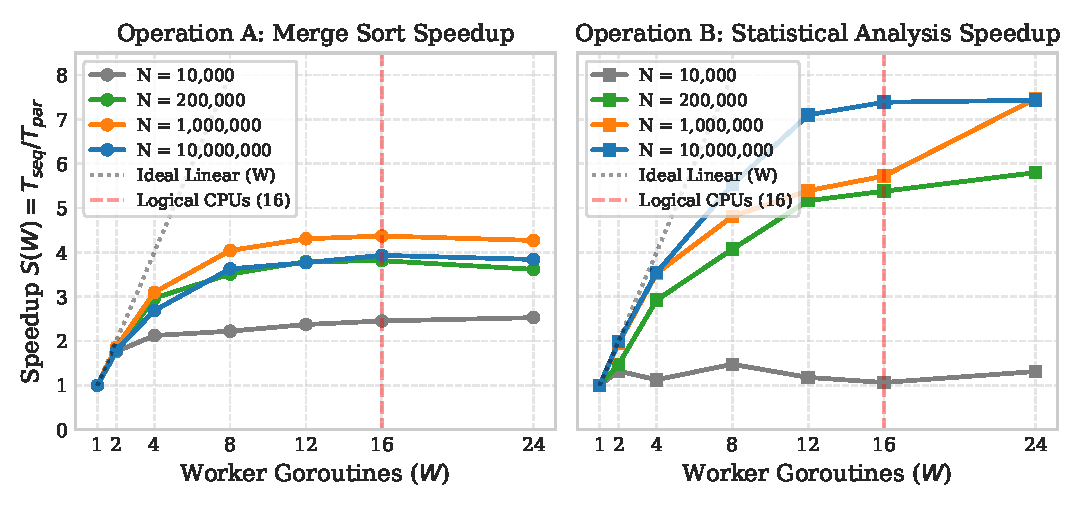
\includegraphics[width=0.96\textwidth]{plot_speedup_workers.pdf}
    \caption{Speedup $S(W)$ vs. Worker Count for Merge Sort (Left) and Stats (Right). Dashed line: 16 logical CPUs.}
    \label{fig:speedup_workers}
\end{figure}

\begin{figure}[h!]
    \centering
    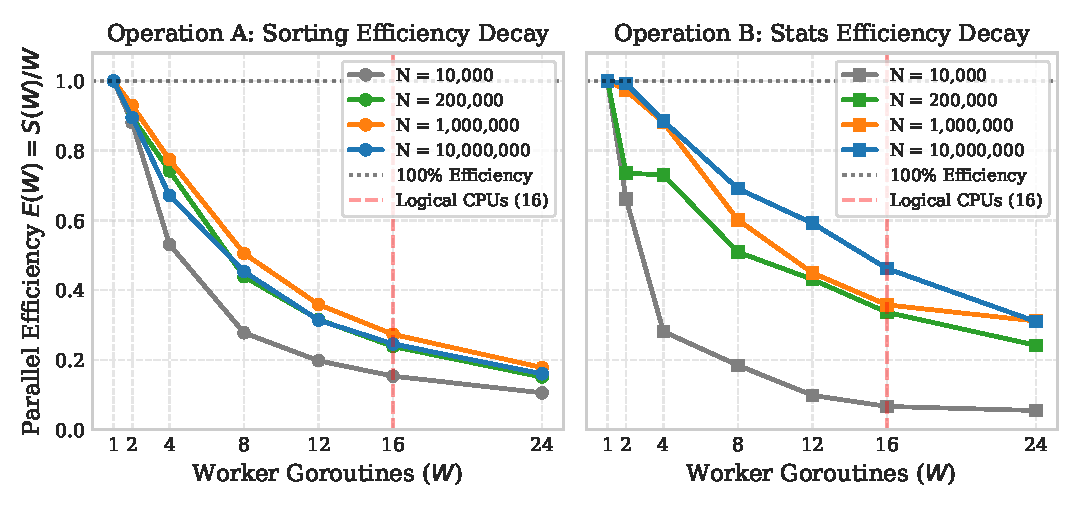
\includegraphics[width=0.96\textwidth]{plot_efficiency_decay.pdf}
    \caption{Parallel Efficiency $E(W) = S(W)/W$ Decay vs. Worker Count for Sorting (Left) and Stats (Right).}
    \label{fig:efficiency_decay}
\end{figure}

\begin{figure}[h!]
    \centering
    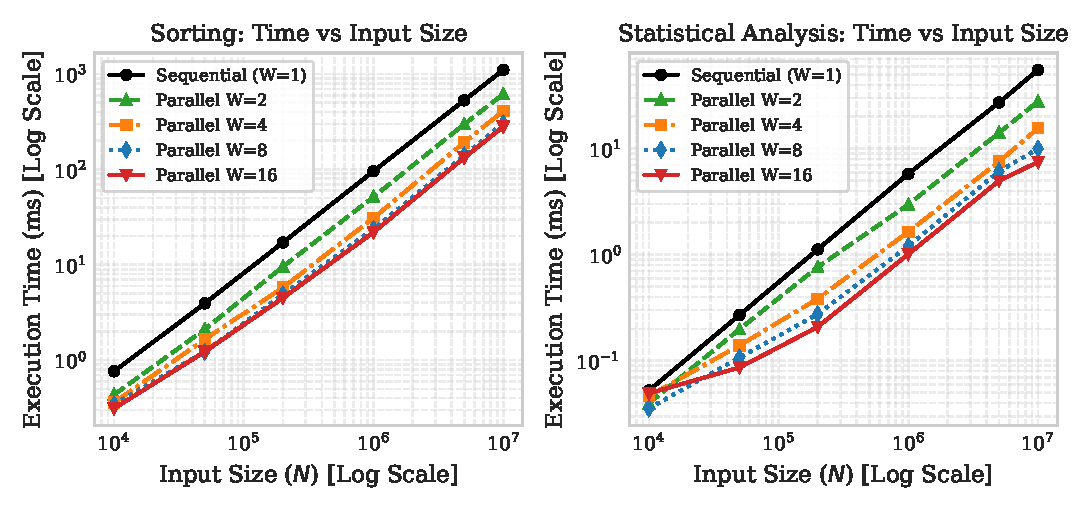
\includegraphics[width=0.96\textwidth]{plot_execution_time_scaling.pdf}
    \caption{Execution Time vs. Input Size $N$ (Log-Log Scale) comparing Sequential vs. Parallel Configurations.}
    \label{fig:execution_scaling}
\end{figure}

\begin{figure}[h!]
    \centering
    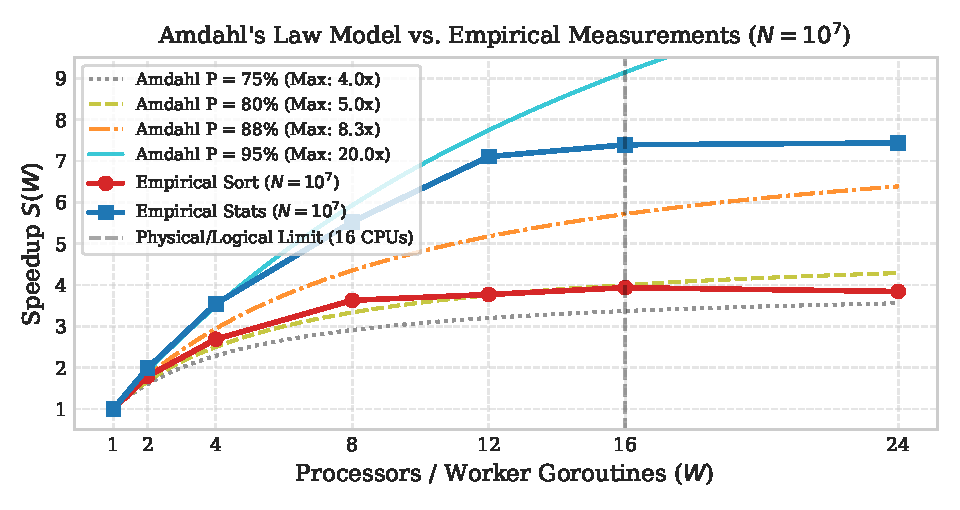
\includegraphics[width=0.82\textwidth]{plot_amdahl_fit.pdf}
    \caption{Amdahl's Law Theoretical Asymptotes vs. Empirical Speedup at $N = 10\,000\,000$.}
    \label{fig:amdahl_fit}
\end{figure}

% --------------------------------------------------------------------------------------------
\newpage

\subsection*{4. Rigorous Investigation of Core Experimental Questions}

\begin{enumerate}[leftmargin=1.6em, itemsep=0.4em]
    \item \textbf{Does parallel execution improve performance for every input size?}\\
    \textbf{No.} For small sizes ($N \le 10^4$), parallel speedup is severely compressed. In isolated single-run testing on $N = 10\,000$ with $W = 8$, parallel sorting required $851\,\mu\text{s}$ compared to $668\,\mu\text{s}$ for sequential sorting ($0.79\times$ speedup, a net slowdown). Goroutine allocation, context switching, and barrier synchronization exceed the computational work saved.

    \item \textbf{Is the improvement proportional to the number of workers?}\\
    \textbf{No.} Scaling is strictly sub-linear and concave. As shown in Figure~\ref{fig:efficiency_decay}, efficiency decays monotonically from $\approx 90\%$ at $W = 2$ to $24.6\%$ at $W = 16$ for sorting. Proportional scaling requires zero coordination and infinite bandwidth, which physical hardware cannot provide.

    \item \textbf{Does either operation become slower after parallelization?}\\
    \textbf{Yes, in two distinct regimes:}
    \begin{itemize}
        \item \textit{Small Workload Regime ($N \le 10^4$):} Microsecond-scale payloads are dominated by thread barrier overhead.
        \item \textit{Over-subscription Regime ($W = 24 > 16$ Logical CPUs):} For $N = 10^7$, sorting execution time degraded from $281.25\,\text{ms}$ at $W=16$ to $287.96\,\text{ms}$ at $W=24$ due to CPU run-queue thrashing and L1/L2 cache evictions.
    \end{itemize}

    \item \textbf{What happens when the number of workers increases beyond logical CPUs?}\\
    When $W > 16$, the Go runtime can no longer map goroutines directly to dedicated OS threads. The OS kernel initiates preemptive involuntary context switches, polluting CPU instruction pipelines and evicting warm cache lines, causing speedup to flatten and regress.

    \item \textbf{Do sorting and statistical analysis exhibit similar scaling behaviour?}\\
    \textbf{No, they diverge fundamentally:}
    \begin{itemize}
        \item \textit{Statistical Analysis scales up to $7.47\times$ speedup} with $99.2\%$ efficiency at $W = 2$. It is an embarrassingly parallel reduction with zero inter-thread communication and a tiny $O(W)$ scalar combination phase ($P \approx 92\%$).
        \item \textit{Merge Sort tops out at $3.93\times$ to $4.37\times$ speedup}. The hierarchical merge tree requires $O(N \log W)$ comparisons and buffer allocations. The final stage merging two $N/2$ arrays into $N$ is inherently serial, imposing an Amdahl bottleneck ($P \approx 78\%$).
    \end{itemize}
\end{enumerate}

% --------------------------------------------------------------------------------------------

\newpage
{\centering\fontsize{14}{17}\selectfont\textbf{Part E --- Correctness Under Concurrency and Concurrency Risks}\par}
\vspace{0.6em}

\subsection*{1. Concurrency Defect Analysis and Architectural Safeguards}
\begin{itemize}
    \item \textbf{Elimination of Shared Mutable State:} In parallel stats, workers write exclusively to their isolated stack frame and store results in a private slice slot \texttt{partialResults[workerID]}, avoiding mutex contention.
    \item \textbf{Partition Boundary Integrity:} The chunking algorithm ensures $\bigcup_{i=0}^{W-1} [S_i, E_i) = [0, N)$ with $E_i = S_{i+1}$, preventing missed or duplicated array indices.
    \item \textbf{Race-Free Merging:} Parallel merge tree routines allocate private buffers \texttt{buf := make([]int, end-start)} and execute on disjoint slice boundaries.
\end{itemize}

\subsection*{2. Race Detector Dynamic Analysis}
The codebase was verified using Go's dynamic ThreadSanitizer race detector:
\begin{lstlisting}[language=bash, caption={Go Race Detector Verification Logs}]
$ go test -v -race
=== RUN   TestSequentialStats               --- PASS: TestSequentialStats (0.00s)
=== RUN   TestParallelStatsEquivalence      --- PASS: TestParallelStatsEquivalence (0.01s)
=== RUN   TestStatsNoMatch                  --- PASS: TestStatsNoMatch (0.00s)
=== RUN   TestSequentialMergeSort           --- PASS: TestSequentialMergeSort (0.00s)
=== RUN   TestParallelMergeSortEquivalence  --- PASS: TestParallelMergeSortEquivalence (0.12s)
=== RUN   TestSortCornerCases               --- PASS: TestSortCornerCases (0.00s)
=== RUN   TestConcurrencyRaces              --- PASS: TestConcurrencyRaces (0.03s)
PASS; ok  assignment06 1.160s

$ go build -race -o analyzer main.go && ./analyzer -mode=verify
SUCCESS: All verification tests passed without errors (0 data races detected).
\end{lstlisting}

\subsection*{3. Concurrency Correctness Principles}
\begin{enumerate}[itemsep=0.3em]
    \item \textbf{Single-Run Success vs. Correctness:} Concurrent execution is non-deterministic. A race condition may execute correctly thousands of times under low contention and fail only under specific OS scheduling delays. Correctness requires formal memory isolation, not single-trial observational success.
    \item \textbf{Silent Data Races:} A data race can occur without producing immediate corrupt output (e.g., atomic cache-line commits on 64-bit words). However, compiler register allocations or architecture changes can trigger latent undefined behavior.
    \item \textbf{Evidence of Correctness:} Our implementation provides: (a) automated mathematical equivalence against sequential baselines; (b) invariant checking via \texttt{IsSorted()}; and (c) dynamic ThreadSanitizer instrumentation reporting zero data races.
    \item \textbf{Limits of Race Detectors:} ThreadSanitizer detects only data races along physically executed code paths during a specific run; it cannot detect logical deadlocks, livelocks, or partition boundary index omissions.
\end{enumerate}

% --------------------------------------------------------------------------------------------
\newpage

{\centering\fontsize{14}{17}\selectfont\textbf{Part F --- Interpretation, Engineering Recommendations, and Reflections}\par}
\vspace{0.4em}
\enlargethispage{3.0\baselineskip}

\subsection*{1. Predictions vs. Experimental Reality}
\begin{itemize}
    \item \textbf{Confirmed:} H1 (parallel sort slower at small $N$), H2 (stats outscaling sort: $7.47\times$ vs $4.37\times$), H3 ($N \ge 10^5$ viability threshold), and H4 (speedup plateau/regression at $W=24 > 16$ logical CPUs).
    \item \textbf{Refined:} Parallel efficiency for statistical analysis dropped to $69.1\%$ at $W=8$ ($N=10^7$), demonstrating that shared memory bus bandwidth saturates earlier than purely compute-bound models predict.
\end{itemize}

\subsection*{2. Production Architecture: Adaptive Dynamic Hybrid Dispatcher}
\noindent\textbf{Context:} Cloud service handling $10^3$ to $10^7$ integer records on shared multi-tenant infrastructure.

\noindent\textbf{Execution Strategy:} The service must \textbf{not} execute statically in parallel. It must dynamically inspect dataset size $N$ and system load:
\begin{itemize}[itemsep=0.2em]
    \item \textbf{Regime 1 ($N < 50\,000$) --- Strictly Sequential Execution ($W = 1$):} Avoids goroutine allocation and barrier overhead, preventing the $21\%$ latency regression observed at small sizes.
    \item \textbf{Regime 2 ($50\,000 \le N < 1\,000\,000$) --- Constrained Parallelism ($W = 4$):} Achieves $\approx 3.0\times - 3.5\times$ speedup at high efficiency ($75\% - 88\%$) without saturating CPU cores.
    \item \textbf{Regime 3 ($N \ge 1\,000\,000$) --- Elastic Parallelism ($W = \min(8, \text{GOMAXPROCS}/2)$):} Drops sorting latency from $1.1\,\text{s}$ to $304\,\text{ms}$ while preserving 50\% of system threads for concurrent tenants.
\end{itemize}

\subsection*{3. Group Reflection Responses}
\begin{enumerate}[itemsep=0.25em]
    \item \textbf{Language Feature vs. Software Design:} Concurrency is fundamentally a software design decision. Programming languages provide syntactic mechanics (e.g., \texttt{go}, channels), but architecture dictates data decomposition, memory barriers, lock freedom, and scaling viability.
    \item \textbf{Non-Proportional Scaling:} Computational scaling is bounded by Amdahl's sequential fraction, memory bus saturation, cache line evictions, and OS context-switch overhead.
    \item \textbf{Complexity vs. Efficiency:} Concurrency introduces synchronization machinery that adds latency. On small problems, this overhead exceeds the work saved, yielding a more complex system that performs worse.
    \item \textbf{Complexity, Parallelism, and Wall-Clock Time:} Algorithmic complexity ($O$) governs asymptotic operations as $N \to \infty$. Parallelism ($p$) divides work across cores. Measured time is physical, dictated by cache hits, memory stalls, and synchronization drag.
    \item \textbf{Production Service Considerations:} (a) Memory churn and GC pressure from scratch buffer allocations (requires \texttt{sync.Pool}); (b) NUMA node memory latency penalties; (c) CFS quota CPU throttling in Docker/Kubernetes; and (d) Graceful cancellation via \texttt{context.Context}.
\end{enumerate}

\subsection*{4. Record of Individual Group Contributions}
\begin{itemize}[itemsep=0.1em]
    \item \textbf{Gaurav Acharya [MT26MCS024]:} Synthesized literature and drafted Part A analytical responses, Task 1 claims, and Amdahl's Law derivations; implemented the sequential baseline and parallel statistical analysis engine; constructed the automated benchmark runner and test suite; led the concurrency risk and race-detection dynamic analysis in Part E.
    \item \textbf{Sandeep [MT26MCS032]:} Designed and implemented the parallel Merge Sort algorithm and hierarchical pairwise merge tree in Part C; built the Python plotting pipeline (\texttt{generate\_plots.py}) and produced the comparative speedup, efficiency, and Amdahl fit figures; conducted benchmarks across all 84 configurations; drafted the production scenario recommendations and final reflections.
\end{itemize}

\end{document}
